% ======================================================================
\section{Computing Randers distances}
\label{app:randers}

\paragraph{Low dimension: eikonal solvers.}
For a fixed source $x_0$, $u=\dF(x_0\to\cdot)$ is the viscosity solution
of the eikonal equation $F^*_x(\nabla u)=1$, $u(x_0)=0$, with $F^*_x$ the
dual norm, again of Randers type by Zermelo's navigation
\citep{bao2000introduction}. Ordered-upwind and adaptive-stencil fast
marching handle asymmetric metrics on a grid
\citep{sethian2003ordered,mirebeau2014efficient}, at $O(N\log N)$ per
source on $N$ nodes and $n$ sources for a full cost matrix. This is
practical in $d=2$ or $3$ only.

\paragraph{High dimension.}
A grid with $m$ nodes per axis has $m^d$ nodes. Graph substitutes run
Dijkstra's algorithm on a directed kNN graph with local Randers edge
lengths, as Isomap does for Euclidean geodesics
\citep{tenenbaum2000global}; heat-kernel proxies replace the infimum by a
small-time limit of a diffusion. Both converge only as the samples
densify around the optimal paths, and both are biased towards dense
regions.

\paragraph{The drift is only sampled.}
The infimum ranges over paths through regions where $\omega$ is not
measured, so its value depends on how $\omega$ is extended between
samples. That is a modelling choice the data do not support.

\paragraph{Proof of \cref{prop:approx}.}
\emph{(1)} Let $g(t)=\omega(x+t\Delta)^\top\Delta$ with $\Delta=y-x$, so
$\ell(x,y)=r+\int_0^1g$. The frozen form replaces $\int_0^1g$ by $g(0)$,
with error at most $\tfrac12\sup|g'|\le\tfrac12L_1r^2$; the averaged form
by $\tfrac12(g(0)+g(1))$, the trapezoid rule, with error at most
$\tfrac1{12}\sup|g''|\le\tfrac1{12}L_2r^3$.
\emph{(2)} \tbd{Make rigorous.} $\ell\ge\dF$ since the segment is one of
the paths. Let $\gamma$ be any path from $x$ to $y$ with Euclidean length
$r+e$ and maximal distance $h$ to the segment. Its Randers length minus
$\ell$ is $e+\oint_\sigma\omega\cdot dx$, where $\sigma$ is the closed
loop $\gamma$ followed by the reversed segment. By Stokes' theorem the
loop integral is bounded by $\tfrac12L_c$ times the area of a surface
spanning $\sigma$, at most $(r+e)h$ for the cone from $x$. A path that
deviates by $h$ has $e\ge c_0\min(h,h^2/r)$. Hence the Randers length of
$\gamma$ is at least $\ell+c_0\min(h,h^2/r)-\tfrac12L_c(r+e)h$; for
$L_cr\le c'$ the minimum over $h$ and $e$ is at least $\ell-cL_c^2r^3$.
\emph{(3)} For $\omega=\nabla\phi$ the drift integral along any path is
$\phi(y)-\phi(x)$, and the Euclidean length is minimised by the segment.

\paragraph{Numerical check.}
\tbd{Table: Study A (experiments/ot), relative errors of the two forms on
gradient drifts in $D=50$ against the exact distance, as a function of
$\|\omega\|$ and neighbourhood size.}

% ======================================================================
\section{Proofs for \cref{sec:gauge}}
\label{app:proofs}

\begin{lemma}[Structure of $\Sep$]
  $\Sep=\{(s_i+s_j)_{ij}:s\in\R^n\}\oplus\Grad$ and $\Sep\cap\Asym=\Grad$.
\end{lemma}
\begin{proof}
  Write $f_i+g_j=(s_i+s_j)+(\psi_j-\psi_i)$ with $s=\tfrac12(f+g)$ and
  $\psi=\tfrac12(g-f)$; the first term is symmetric and the second
  antisymmetric, so the sum is direct. If $f_i+g_j$ is antisymmetric, its
  diagonal gives $g=-f$, hence $f_i+g_j=f_i-f_j\in\Grad$.
\end{proof}

\begin{proof}[Proof of \cref{thm:identifiability}]
  The kernel is entrywise positive, so the scaling exists and the coupling
  is unique \citep{sinkhorn1967concerning}. If $C'_{ij}=C_{ij}+f_i+g_j$,
  then $e^{-C'/\eps}=\diag(e^{-f/\eps})\,e^{-C/\eps}\diag(e^{-g/\eps})$;
  the diagonal factors are absorbed into the scalings, and uniqueness gives
  the same coupling. Conversely, if both couplings equal $P$, then
  $\log P_{ij}=\log u_i+\log v_j-C_{ij}/\eps=\log u'_i+\log v'_j-C'_{ij}/\eps$,
  so $C-C'\in\Sep$. The second statement follows from the lemma.
\end{proof}

\paragraph{Cyclic part.}
Adding $G\in\Grad$ to $A$ shifts the minimiser in the definition of
$\cyc_W$ by $G$, so $\cyc_W(A+G)=\cyc_W(A)$; conversely, equal cyclic parts
force $A-A'$ to be a difference of minimisers, a gradient. The normal
equations give $\sum_jW_{ij}\cyc_W(A)_{ij}=0$ for every $i$.

\paragraph{Net flow.}
If $P\1=P^\top\1=a$, then $\sum_{ij}P_{ij}(f_j-f_i)=\sum_ja_jf_j-\sum_ia_if_i=0$.
Taking $f=\1_k$ gives $((P-P^\top)\1)_k=0$. The chain $\diag(a)^{-1}P$ has
stationary law $a$, and so do its powers.

\paragraph{An optimal transport reading.}
On couplings with marginals $a,b$,
$\sum_{ij}P_{ij}(C_{ij}+f_i+g_j)=\langle P,C\rangle+\langle a,f\rangle+\langle b,g\rangle$:
a separable change of cost shifts every transport cost by the same
constant and leaves optimal plans unchanged, with or without entropy.
For an exact gradient drift, unregularised OT under the Randers cost
therefore has the optimal plans of the Euclidean $W_1$ problem. The
converse of \cref{thm:identifiability} needs entropy: an unregularised
plan constrains the cost only through cycle sums.

% ======================================================================
\section{Hodge decompositions}
\label{app:hodge}

\begin{figure}[h]
  \centering
  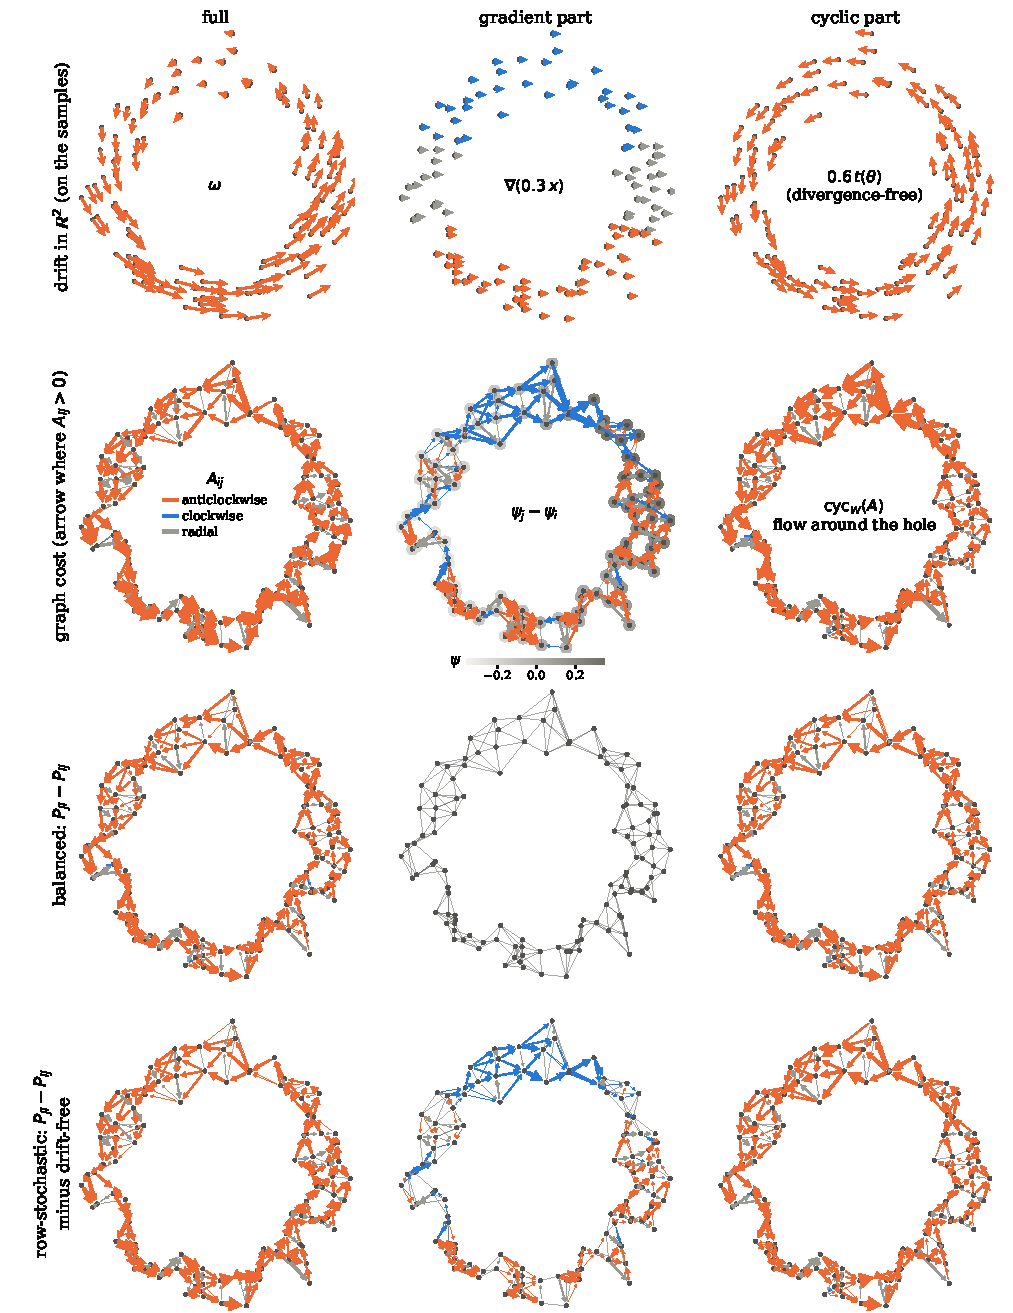
\includegraphics[width=0.7\textwidth]{figures/hodge_ring.pdf}
  \caption{Weighted Hodge decomposition on a ring (120 points, symmetrised
  5-NN graph, linear cost, global bandwidth). The drift is
  $\omega=0.6\,t(\theta)+0.3\,e_x$, a rotation, which is harmonic on the
  ring, plus a uniform drift, an exact gradient. Columns: full, gradient
  part, cyclic part. Rows: the drift in $\R^2$; the graph cost
  $A_{ij}$, arrow $i\to j$ where $A_{ij}>0$, width $\propto|A_{ij}|$,
  coloured by orientation around the ring; the balanced affinity's net
  transport $P_{ji}-P_{ij}$, which carries no gradient part; the
  row-stochastic one's, minus that of the drift-free affinity, which
  carries both.}
  \label{fig:hodge_full}
\end{figure}

\paragraph{Real velocity fields.}
\label{app:hodge_data}
\tbd{Table: gastrulation ($n=30\,000$, 30-NN graph in 30-PC space):
gradient share 0.75--0.83 (null 0.31--0.33), and a walk on the cyclic part
alone gains no days; RPE1-FUCCI ($n=2793$): gradient share 0.67 for the
direct velocity, but its gradient part walks backwards around the cycle
($-0.06$ cycle after 25 steps) while the curl part advances ($+0.26$).}

% ======================================================================
\section{What the output loss rewards}
\label{app:output}

\tbd{Test 1 of experiments/theory/output\_kernel.py: first-order loss
sensitivity at the symmetric fit to gradient vs rotated perturbations of
the output drift, Student and Laplace kernels, pancreas and RPE1, balanced
and row-stochastic inputs, $q=2$ and $q=1$. Exact cancellation for the
Laplace kernel with an exact potential cost ($10^{-14}$).}

% ======================================================================
\section{Implementation details}
\label{app:implementation}

Both Randers affinities accept any backend of TorchDR.

\paragraph{Costs from matrix products.}
The drift term of \eqref{eq:averaged} rearranges to
\[
  A_{ij}=\tfrac12\big[(\Omega X^\top)_{ij}-(X\Omega^\top)_{ij}+s_j-s_i\big],
  \qquad s_i=\omega_i^\top x_i ,
\]
with $\Omega$ the matrix of drifts, so the cost needs $(n,n)$ products and
never the $(n,n,D)$ tensor of differences: at $n=2000$, $D=100$, this is
$100\times$ faster (0.07~s against 7.5~s) and avoids a 3.2~GB tensor.

\paragraph{Linear memory with KeOps.}
With KeOps \citep{charlier2021keops}, the output cost \eqref{eq:Q} is a
symbolic lazy tensor: the normaliser $\sum_{k\neq l}(1+\dav_\theta^2)^{-1}$
and its gradients are reduced on the fly, in $O(n)$ memory. The input
affinity is made sparse by keeping, in each row, the $k=5\mathcal{P}$
nearest points under the \emph{directed} cost, found by a KeOps
$\arg\min_k$; the loss \eqref{eq:loss} then splits into an attraction on
the $nk$ kept entries and the lazy normaliser. Dense and KeOps paths agree
to $10^{-15}$ in float64 on losses and gradients.

\paragraph{Sinkhorn.}
A per-row perplexity bandwidth makes the balanced kernel badly
conditioned: thousands of iterations are needed to reach marginal errors
below $10^{-4}$. We run Sinkhorn in the log domain, in float32 if needed,
with early stopping on the marginal error. On kNN-sparse inputs we balance
the kNN graph with its reverse edges; this is a local variant of balancing
rather than an approximation of the dense one, so we use row-stochastic
affinities at scale.

\begin{table}[h]
  \caption{Time per optimisation step (loss, backward, Adam step) and peak
  memory, RTX 2080 Ti, float32, $k=250$. Dense runs are skipped when they
  would exceed the GPU's memory.}
  \label{tab:scaling}
  \centering
  \small
  \setlength{\tabcolsep}{4pt}
  \begin{tabular}{rcccc}
    \toprule
    $n$ & input aff. & KeOps step & memory & dense step \\
    \midrule
    $10^4$ & 1.7~s & 0.020~s & 0.26~GB & 0.097~s \\
    $2\cdot10^4$ & 2.4~s & 0.034~s & 0.49~GB & -- \\
    $5\cdot10^4$ & 8.1~s & 0.112~s & 1.21~GB & -- \\
    $10^5$ & 19.9~s & 0.359~s & 1.73~GB & -- \\
    \bottomrule
  \end{tabular}
\end{table}

\paragraph{Performance.}
\Cref{tab:scaling} shows the scaling: memory grows linearly, and a
3000-step fit of $10^5$ points takes about 18 minutes on a consumer GPU.
Quality holds at scale: on a synthetic vortex with $n=5\cdot10^4$, the
fitted speed correlates at $0.94$ with the true one (against $0.89$ at
$n=1500$), provided the perplexity grows as $\sqrt n$; capping it at $50$
halves the cost but drops the correlation to $0.82$.

% ======================================================================
\section{Architectures that did not help}
\label{app:architecture}

\tbd{Short summary with numbers from experiments/toy/stream\_sphere.py:
a $64\times2$ MLP matches the $32\times1$ one; random Fourier features
improve direction slightly at the same loss; a divergence-free drift
$\omega=J\nabla h$ loses 40--60\% of the loss gain and folds the layout,
because a push-forward under a map that does not preserve area is not
divergence-free; an exact potential drift ($\omega=\nabla h$) gives
slightly worse layouts than the symmetric fit.}

% ======================================================================
\section{Synthetic flows: details}
\label{app:toy}

\tbd{Protocol (Adam learning rates, iterations, $\rho$, perplexity),
vortex-centre analysis of the sphere fits (experiments/toy/stream\_sphere.py
poles), and the figure of all layouts.}

\paragraph{Why the ring folds.}
\label{app:fold}
On the noisy cycle every direction-blind layout (symmetric t-SNE of the
same affinity, Finsler MDS, Isomap) draws the ring as a convex loop, and
every FlowSNE joint fit as a thin meandering line (\cref{fig:toy_layouts}).
\Cref{tab:fold} scores the ring's shape by the convexity of the polygon
through its 24 phase-bin centroids (area over convex-hull area) and by its
total turning in units of $2\pi$; a convex loop scores $1$ on both. The
optimiser schedule is not the cause: early exaggeration, a cosine learning
rate, a ten times smaller rate for the flow and a warm-up leave the shape
unchanged. Nor is the lift: with a linear lift to $\R^{50}$ (no sine
features) the ring folds the same. The cause is the objective. A drift of
norm $|\omega|$ makes a forward step of length $r$ cost $(1-|\omega|)r$,
so to reproduce the input's affinity decay the joint fit stretches the
layout along the flow and thins it: the ring's perimeter relative to the
layout's r.m.s.\ radius is $5.2$--$5.4$ for the symmetric layouts
($2\pi$ for a circle), $8.3$--$8.5$ for the joint fits, and its
transverse width halves. A stretched loop in the plane meanders. Lowering
the bound to $\rho=0.5$ halves the stretch ($6.4$) and nearly unfolds the
ring, but the field can no longer rank speeds. A warm start from the
symmetric layout, instead of PCA, reaches a lower loss than the PCA start
on every seed, with a rounder ring and the same direction and speed: the
PCA-started fit settles in a more folded local minimum. The exact circle
with the best field fitted on it has the highest loss of all
($11.55$): the loss genuinely prefers some bending.

\begin{table}[h]
  \caption{Noisy cycle, seed 0 (warm start: 3 seeds), balanced / row-stochastic input.
  Direction, speed and loss as in \cref{tab:toy}; conv.\ and turn: ring shape (1 = convex loop).}
  \label{tab:fold}
  \centering
  \small
  \setlength{\tabcolsep}{3pt}
  \begin{tabular}{lccccc}
    \toprule
    joint fit & dir. & speed & loss & conv. & turn \\
    \midrule
    symmetric layout (no drift) & -- & -- & -- & 1.00 / 1.00 & 1.04 / 1.01 \\
    PCA start (\cref{tab:toy}) & 0.95 / 0.98 & 0.53 / 0.75 & 11.41 / 11.43 & 0.67 / 0.66 & 2.7 / 2.6 \\
    \quad + exagg., cosine, flow lr, warm-up & 0.95--0.96 / 0.97--0.98 & -- & 11.41--11.53 & 0.66--0.70 / 0.62--0.70 & 2.6--2.8 \\
    \quad with $\rho=0.5$ & 0.94 / 0.97 & $-0.20$ / 0.37 & 11.51 / 11.56 & 0.88 / 0.89 & 1.6 / 1.6 \\
    \quad linear lift, no sines & 0.83 / 0.98 & 0.42 / 0.63 & 11.38 / 11.42 & 0.67 / 0.62 & 2.4 / 2.6 \\
    warm start from symmetric layout & 0.96 / 0.98 & 0.62 / 0.78 & 11.33 / 11.36 & 0.76 / 0.83 & 2.3 / 2.2 \\
    \quad with $\rho=0.7$ & 0.95 / 0.97 & 0.47 / 0.49 & 11.39 / 11.44 & 0.90 / 0.94 & 1.5 / 1.5 \\
    field fitted on the frozen circle & 0.93 / 0.88 & $-0.25$ / $-0.06$ & 11.55 / -- & 1.00 & 1.0 \\
    \bottomrule
  \end{tabular}
\end{table}

